\section{App Management}
\label{sec:app_management}
\label{sec:appman_solution}
\label{sec:appman_requirements}

When the user launches a \giraf[] app, the transitions between \emph{No app selected} and \emph{No child selected}, are taken, as seen in \autoref{fig:state_diagram}.\\

\noindent Three pieces of information are needed in order to launch an app:

\begin{enumerate}
	\item Current authenticated guardian
	\item App to launch
	\item Selected child profile to launch the app for
\end{enumerate}

The first requirement is already given, since the launcher cannot be in any of the two states without the user already being authenticated.
The second requirement is given, as it is not possible to launch an app without knowing which app to launch.
The first and third requirements are needed in order to fulfill the services which the launcher needs to have in order to be a functional part of the \giraf[] platform, as shown in \autoref{fig:external_architecture}.

Furthermore, additional pieces of information are available:

\begin{enumerate}
	\item Date related data
	\item Network status 
\end{enumerate}

As the \giraf[] platform is thought to be the primary electronic tool of guardians, date related data is provided. Date related data is thought to be the day in characters the day in number, the month in characters and the week number. Later date related data can be a calendar app if such an app is installed on a device running \giraf[].
Since the \giraf[] platform uses both local and remote storage, there might be latency in synchronizing these storages.
It is therefore important for the user to know if both storages are synchronized.

\autoref{fig:appmanagement_design} shows a flow chart of the interactions the user can perform, and the actions the launcher takes upon the interactions, in order to fulfill the requirements listed earlier.\\

\begin{figure}[!h]
	\centering
	\includegraphics[width=1\textwidth]{gfx/appmanagement.pdf}
	\caption{Flow chart over the app management functionality}
	\label{fig:appmanagement_design}
\end{figure}

\autoref{fig:appmanagement_design} shows three branches of user interactions and system actions:


\paragraph{Drawer} For a user to change app settings, he or she must open the drawer, a component explained below. 
In the drawer, there is a color picker, also explained later, from which the user chooses a color and drags it to the desired app. 
The user can ``cancel'' the color change at any point, either by not choosing a color, or releasing the color over something that is not an app. 

\paragraph{Apps} When launching an app, the user chooses an app to launch and clicks it. 
This brings the launcher out of \emph{App Management}, and into \emph{Profile Selection}, explained later. 
The user can ``cancel'' the action by not choosing an app.%, or by coming back to \emph{App Management} after it has been left.

\paragraph{Widgets} Finally, the user can request information, which happens through widgets, explained below. 
There are different widgets in the system, and every widget contains unique information.
The user chooses which one to recieve information from, and clicks the widget containing the desired information to have it shown. 
If the user does not choose a widget, the action is cancelled. 

\subsection{Drawer}
\label{sec:drawer}
As stated, the drawer was designed to hide functionality, that is not always needed, in a convenient place. 
As seen in \autoref{fig:appmanagement_design} everything that has to do with changing app settings is placed in the drawer, and the user has to open the drawer to get to this functionality.
The drawer is shown in \autoref{fig:design_prototype} in context.

\begin{figure}[!h]
	\centering
	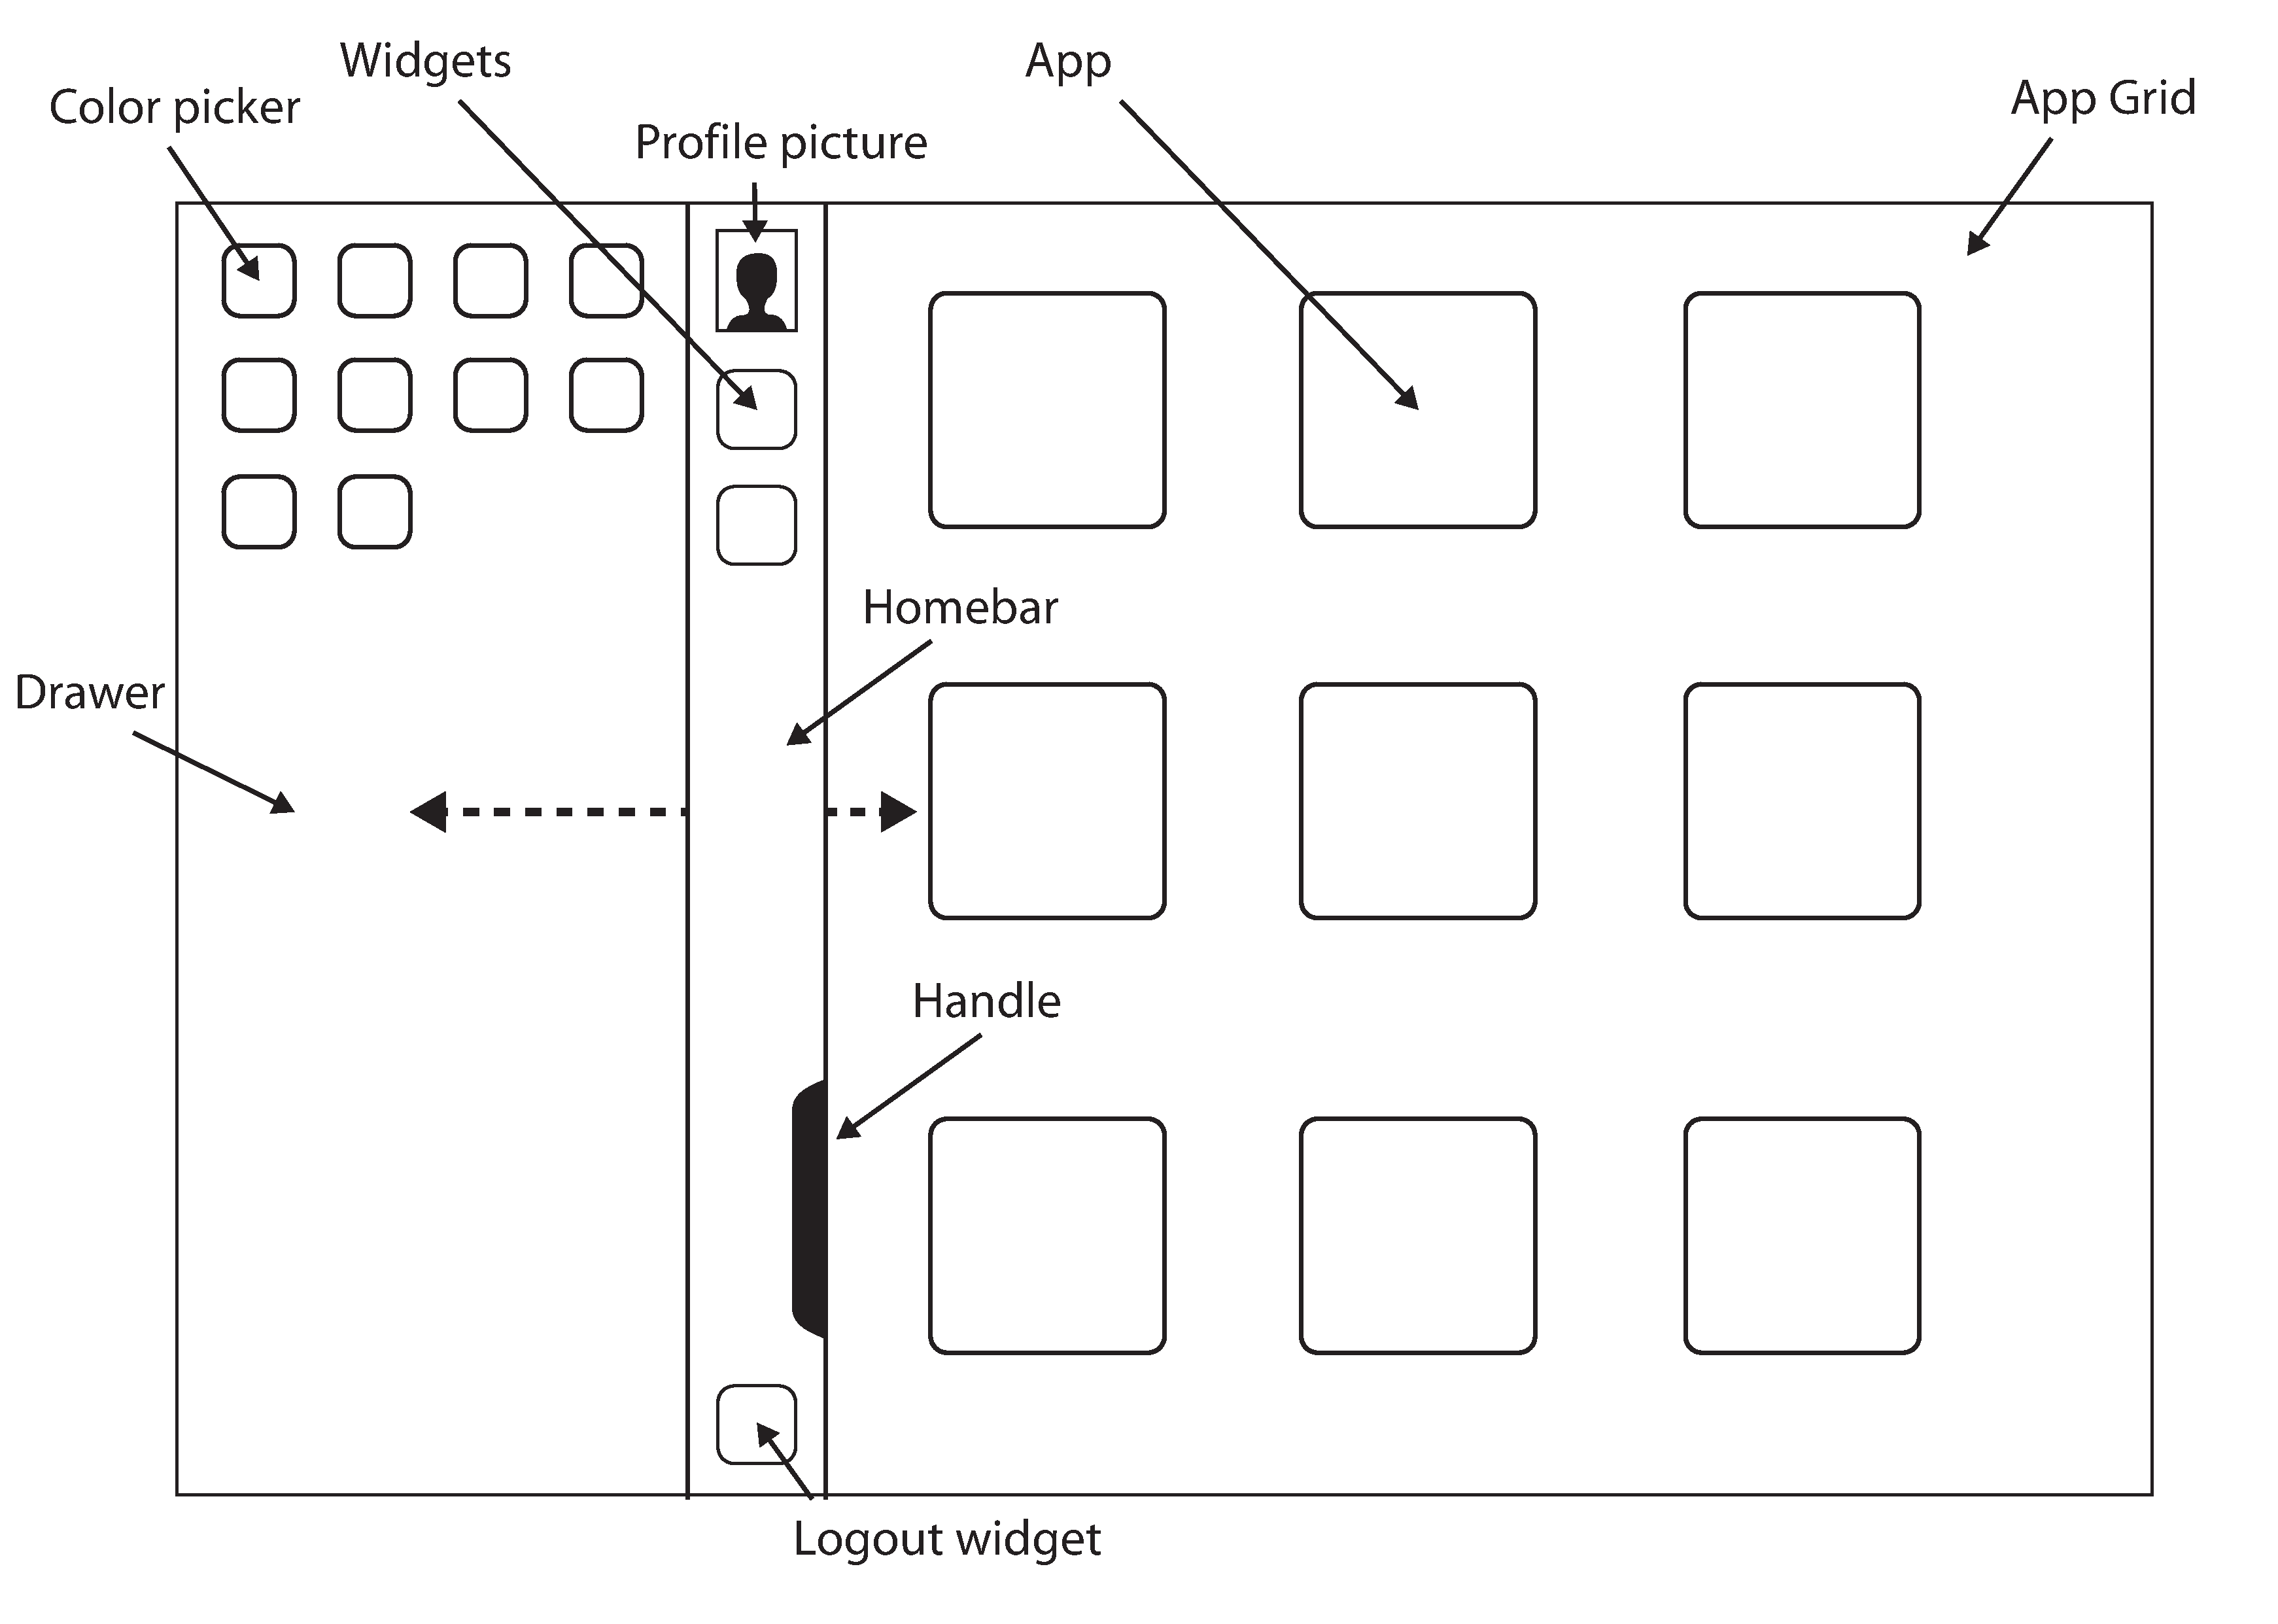
\includegraphics[width=1\textwidth]{gfx/design_prototype.pdf}
	\caption{Illustration of the app management components}
	\label{fig:design_prototype}
\end{figure}

\begin{figure}[!h]
	\centering
	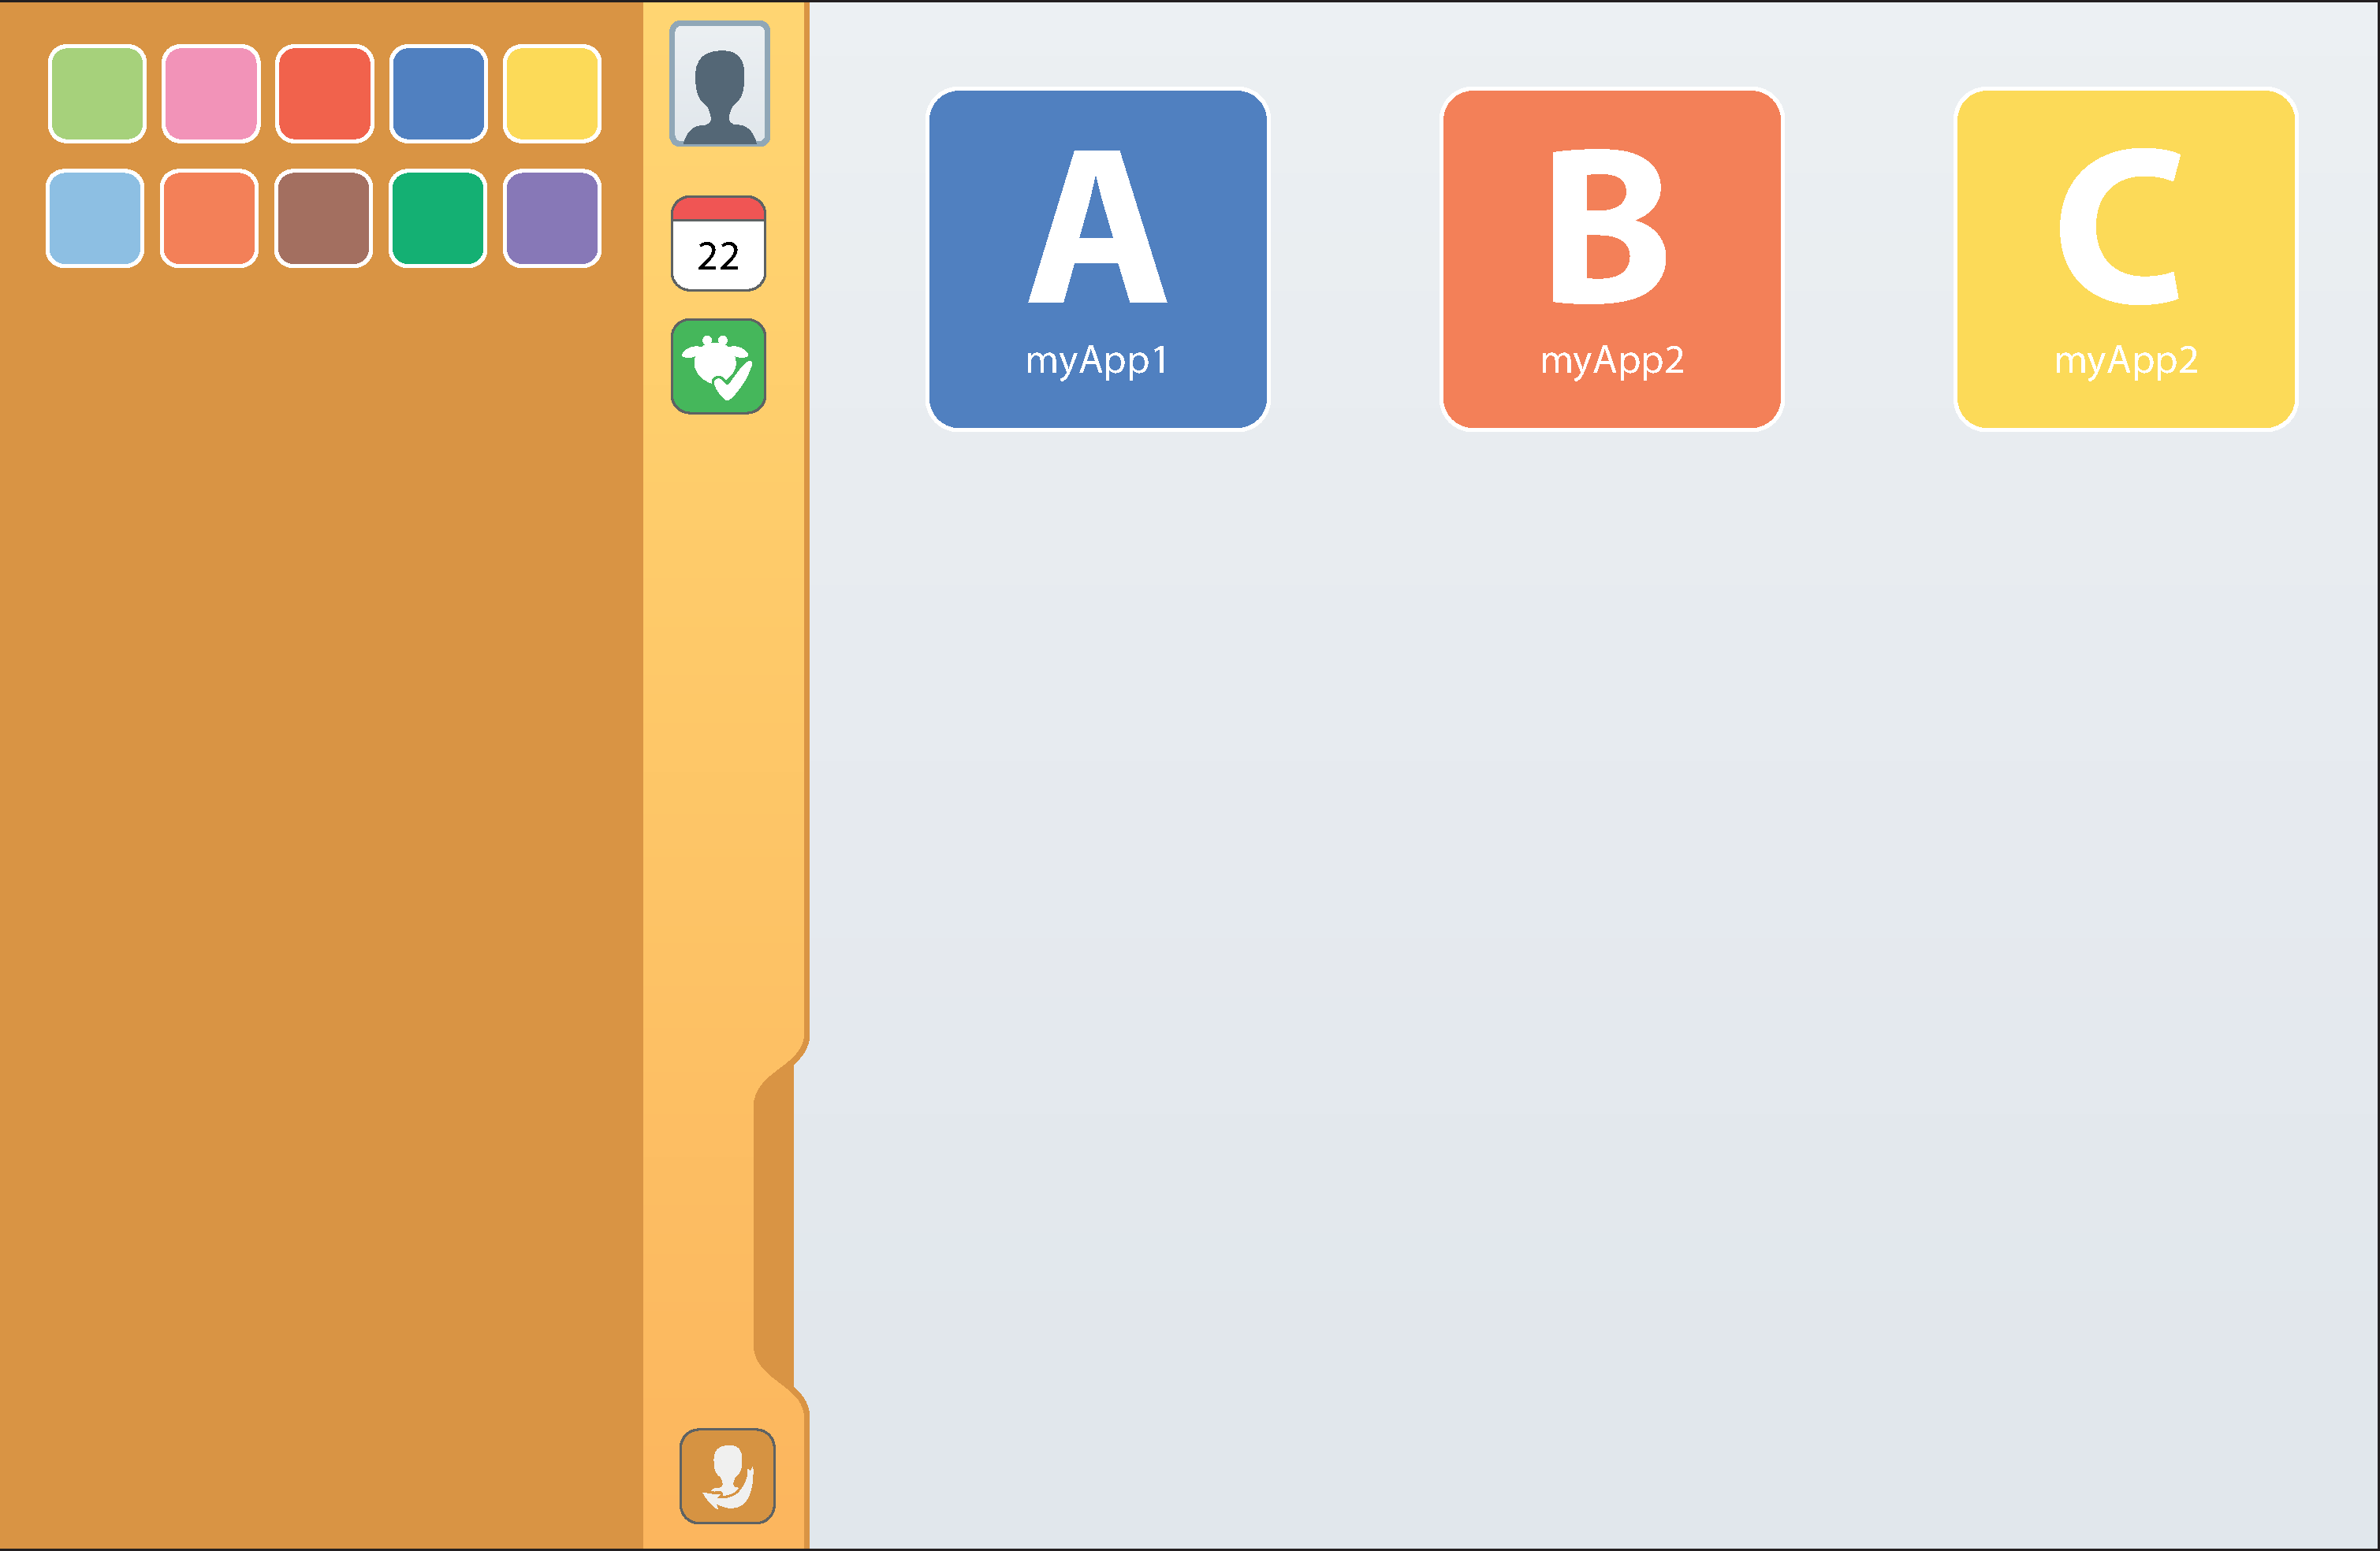
\includegraphics[width=1\textwidth]{gfx/gui_appmanagement_open.pdf}
	\caption{Design of app management, with drawer opened}
	\label{fig:gui_appmanagement_design}
\end{figure}

To highten consistency, the handle and the inside of the drawer have the same color.
The handle has rounded corners, see \autoref{design:button_design}, to tell the user that this element is interactive.
An illustration with the drawer closed can be seen in \autoref{fig:gui_appmanagement_closed_design}, and one with the drawer open in \autoref{fig:gui_appmanagement_design}.

\begin{figure}[!h]
	\centering
	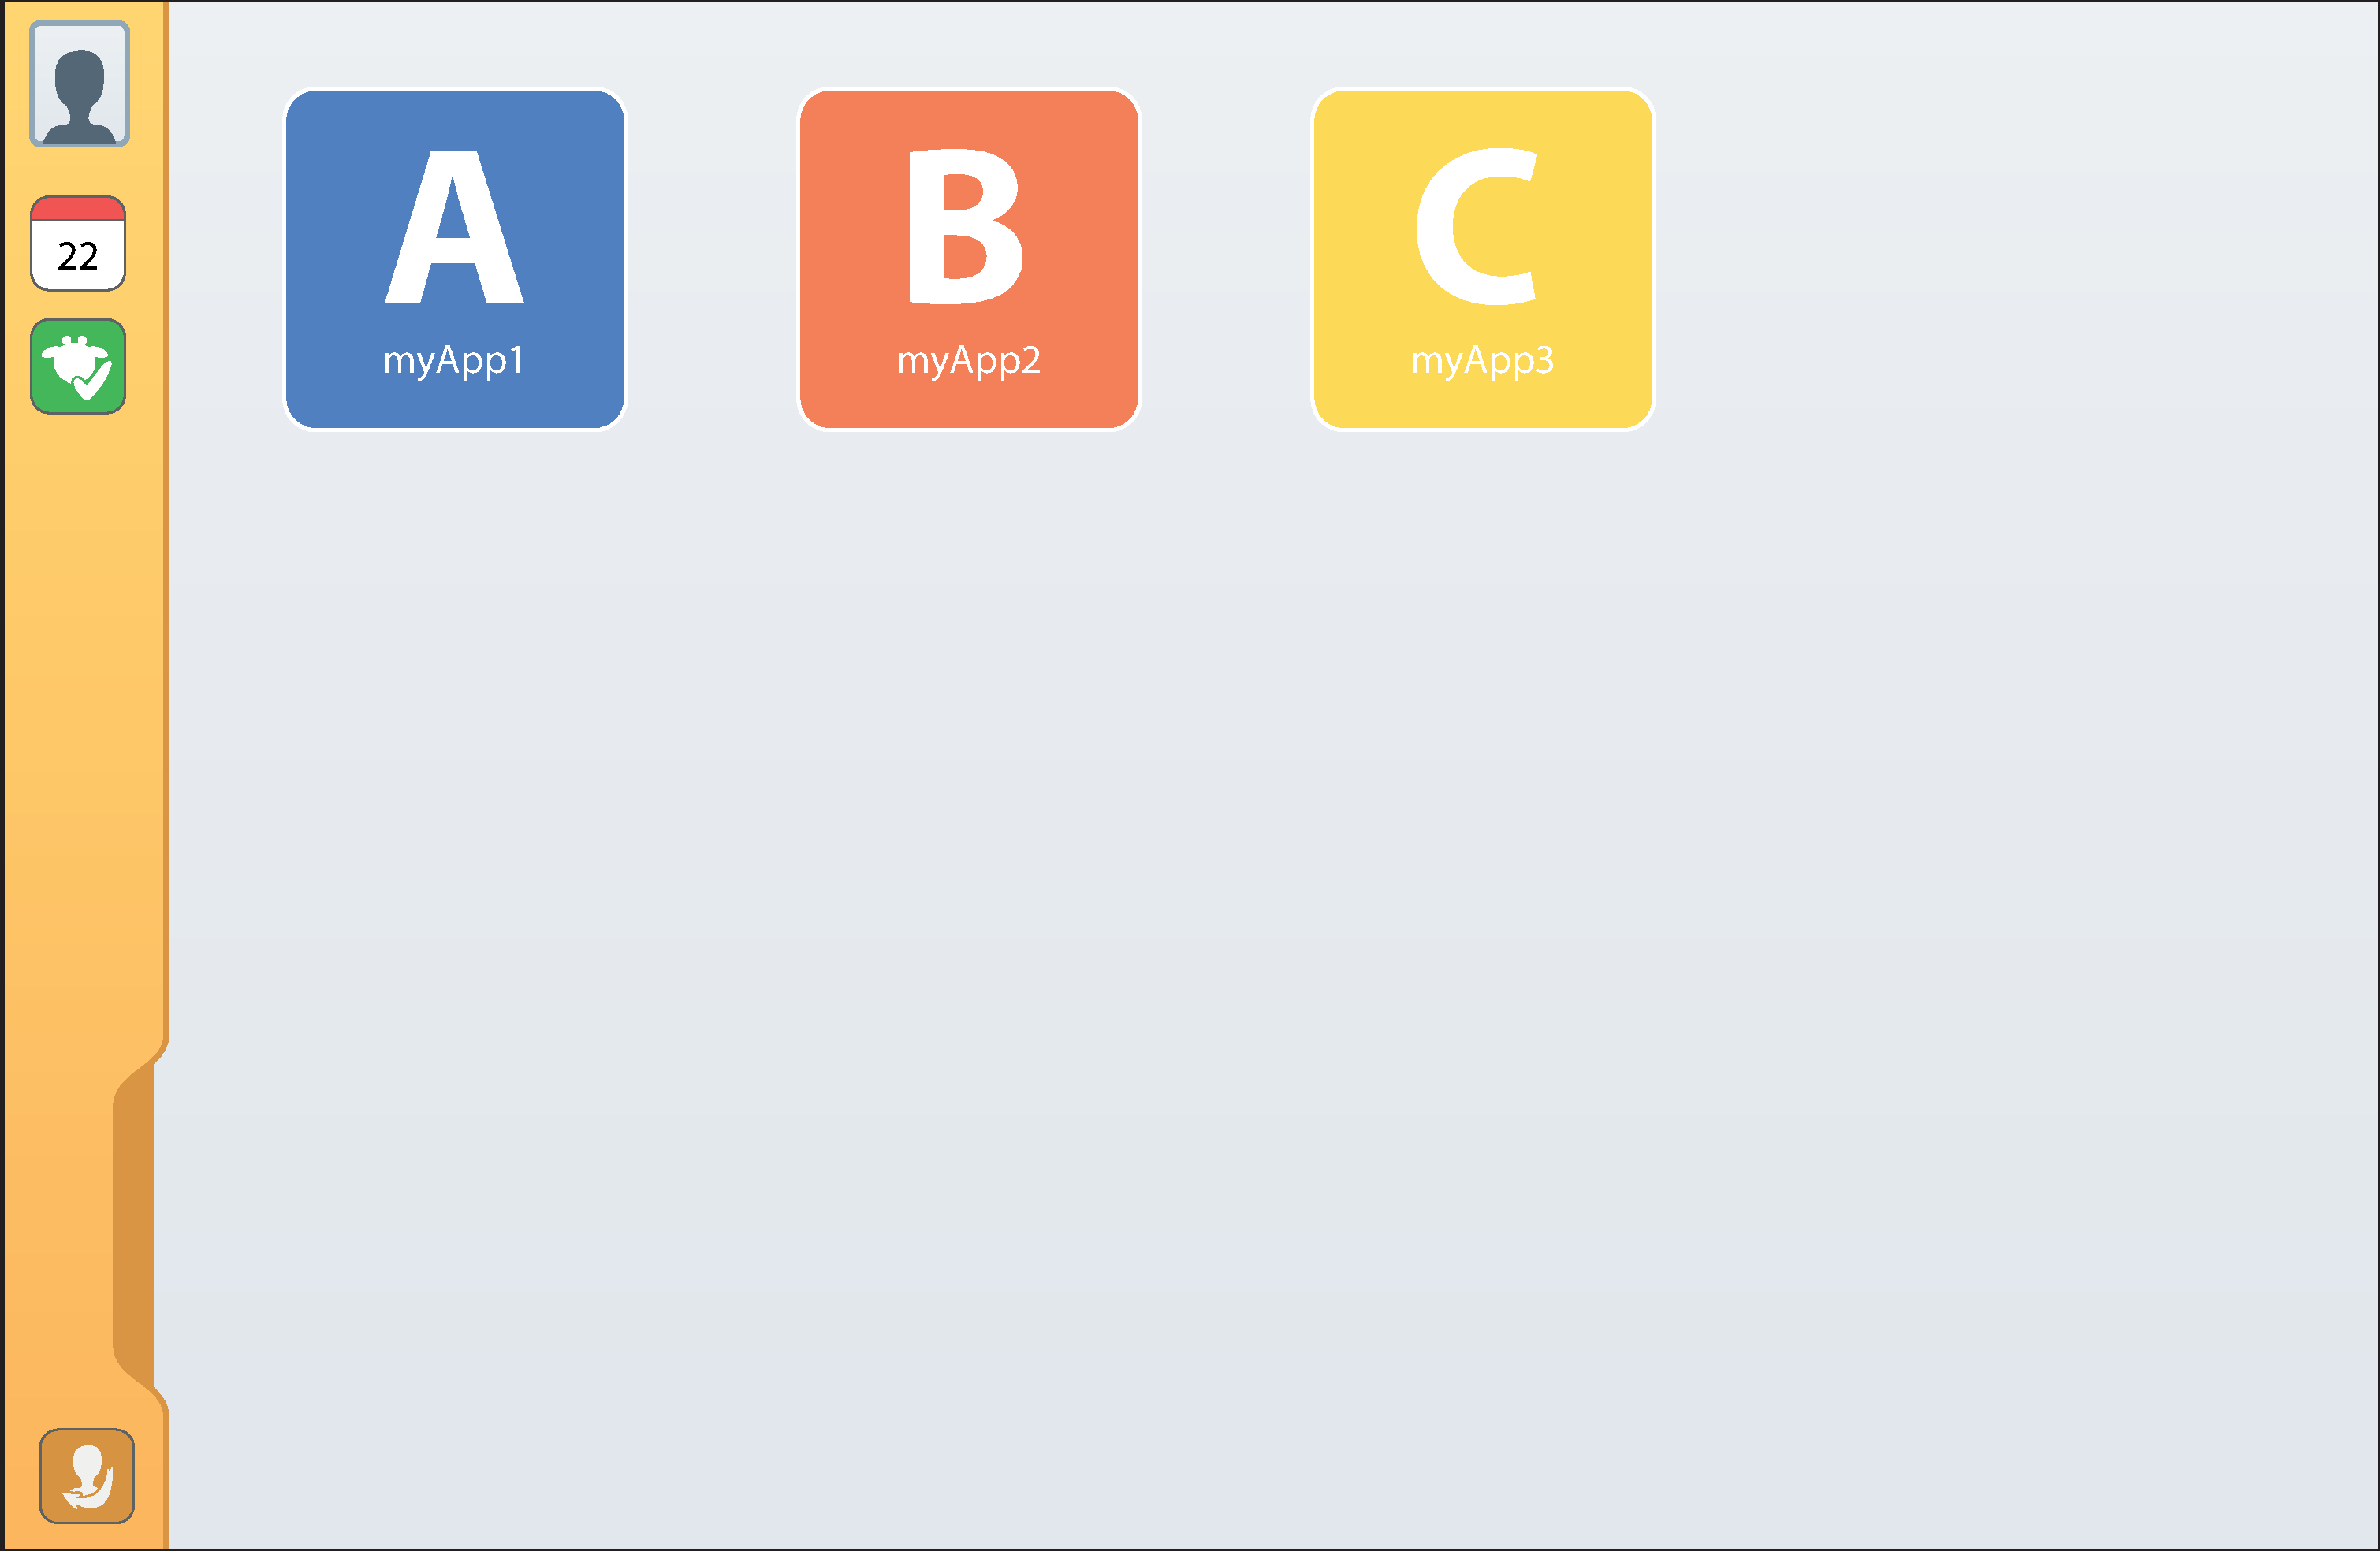
\includegraphics[width=1\textwidth]{gfx/gui_appmanagement_closed.pdf}
	\caption{Design of app management, with drawer closed}
	\label{fig:gui_appmanagement_closed_design}
\end{figure}

\subsubsection{Widgets}
\label{par:widgets}
Widgets in the \giraf[] system are used to display information to the user, and might let the user take an action.  
An action can e.g. be to present additional information to the user, or to produce a side effect in the system. 
\autoref{fig:design_prototype} shows the placement of the widgets in context.

All widgets are designed with round corners to signal interactivity, in accordance with \autoref{design:button_design}.
The widget \emph{logout} is kept seperately from the other widgets, as it allows the user to change the state of the launcher to \emph{No credentials provided}, as seen in \autoref{fig:state_diagram}, while the other widgets keep the launcher \emph{No app selected}.
The widgets can be seen in \autoref{fig:gui_appmanagement_design}.

\subsubsection{Color picker}
\label{par:colorpicker}
All colors in the color picker have rounded corners as they are interactive.
They have white edges to keep them distinguishable from the background.
The color picker consists of ten predefined colors. 
The reason for using predefined colors in the color picker is to ensure contrast. 
If developers of \giraf[] apps make their app icons mono-colored white, the contrast would always be sufficient. 
This should ensure that users will be able to see the icon, no matter what icon background color was chosen.

\autoref{fig:design_prototype} shows the placement of the color picker in context, and \autoref{fig:gui_appmanagement_design} shows the complete graphical design.